\section{Experimental Setup}
\label{sec:exp_setup}

We have implemented our algorithm \textit{MsgSchedModule} for adaptive message scheduling with ECN and varying $\delta$ support using C++ in linux environment. Boost portable C++ source libraries~\cite{boost} were used for timing needs in our \textit{MsgSchedModule}. Network was emulated using OMNet++, an open source network simulator ~\cite{omnet, omnetpaper}. OMNet++ is a discrete event simulator that provides an extensible, modular, component-based C++ simulation library. OMNet++ also supports emulation of network in real time instead of just being a simulator~\cite{mayeromnet}. Real-time scheduler class \textit{cRealTimeScheduler()} in OMNet++ was used in our network emulation.
Figure~\ref{fig:dgi_net} shows the network setup used to emulate every power transfer phase. Nodes (denoted as \textit{realPeer50} and \textit{simPeer0} to \textit{simPeer8}), communicate with each other over links and routers (\textit{router0} to \textit{router5}). Nodes are also capable of generating traffic in the network. Note that \textit{MsgSchedModule} is an external module which connects to \textit{realPeer50} through socket to \textit{localhost} at configured \textit{port}. In this paper, we experiment using \textit{realPeer50} as an excess power node. Routers employ first-in-first-out (FIFO) queue with configurable service time $Q_{st}$ for every (total 4 ports) outgoing port. 
Routers being ECN capable, maintain queue average $Q_{avg}$, check $Q_{avg}$ against $Q_{min}$ and $Q_{max}$ thresholds and set congestion experienced (CE) bit in messages if required. Note that $Q_{min}$, $Q_{max}$ and $Q_{st}$ are configurable parameters. 
For the current paper experiments, $Q_{min}$, $Q_{max}$ and $Q_{st}$ are set to 3, 20 and 0.2s (seconds) respectively.
In the current paper, we focus on studying the behavior of our \textit{MsgSchedModule} featured with ECN support and varying $\delta$ support versus non ECN support and constant $\delta$. For a given power transfer phase, the required input data for \textit{realPeer50} as $P_G$ (amount of power granted by \textit{realPeer50} to some node, say \textit{simPeer8}), $K_{max}$, $RT_s^{ex}$, $RTMargin$ and $CtrMax$ (for Normal mode, because in ECN mode $CtrMax$ increases in proportion to outstanding messages $K$) is assumed to be available from state information phase (Figure 3).

{\bf System configuration, }\textit{realPeer50} is excess power node, \textit{simPeer8} is the node demanding $20000~units$ of power and $K_{max_{global}}$ is set to 20. Since there is only one node \textit{realPeer50} with excess power in the experimenting power transfer phase, $K_{max}$ for \textit{realPeer50} is 20, i.e \textit{realPeer50} can have maximum of 20 outstanding power transfer messages in the network. Quantum of power $\delta$ is set to $10$ for experiments with constant $\delta$, whereas $\delta$ is allowed to vary between $10$ to $30$ ($\delta_{min}$, $\delta_{max}$) for experiments with varying $\delta$. Route between \textit{realPeer50} and \textit{simPeer8} is through \textit{router0-router2-router4-router5}. To experiment with traffic, \textit{simPeer7} and \textit{simPeer5} communicate with each other through route \textit{router2-router4} and generate messages such that
they occupy \textit{50 percent} of total bandwidth. For all the experiments with traffic, traffic is generated from time $t=5000$ to $t=10000$. 

Considering that \textit{realPeer50} granted $20000~units$ of excess power it has to \textit{simPeer8}, \textit{realPeer50} initializes its local variables as, $P_{G(8)}=20000$, $P_{T(8)}=0$ and $P_{A(8)}=0$. In case of constant $\delta$, whenever \textit{realPeer50} wants to transfer $\delta$ amount of power, invariants $I_S$ and $I_P$ are evaluated, if they return $true$, or are satisfied, then only a power transfer message is dispatched to \textit{simPeer8}. Whereas in varying $\delta$ case, before $I_k$ in $I_S$ is evaluated, \textit{MsgSchedModule} calculates $\delta$ size at that instance of time by Equation 13 and if calculated $\delta$ is greater than $\delta_{max}$ then $\delta$ is set equal to $\delta_{max}$ or if calculated $\delta$ is less than $\delta_{min}$ then $\delta$ is set equal to $\delta_{min}$.

\begin{figure}[htb]
  \begin{center}
    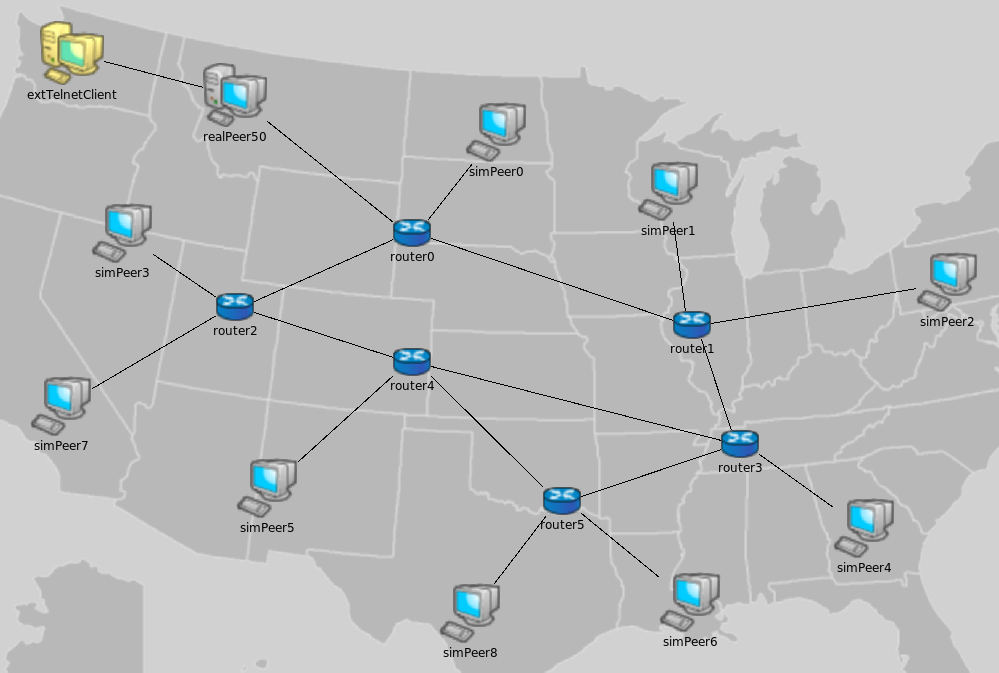
\includegraphics[width=0.50\textwidth]{Figures/iccps2014/dgi_net.png}
  \caption{Emulated Network in OMNet++}
  \label{fig:dgi_net}
  \end{center}
\end{figure}

\subsection{Experimental Results}
\label{sec:exp_results}


%----------------------------------------
\begin{figure}[htb]
  \begin{center}

    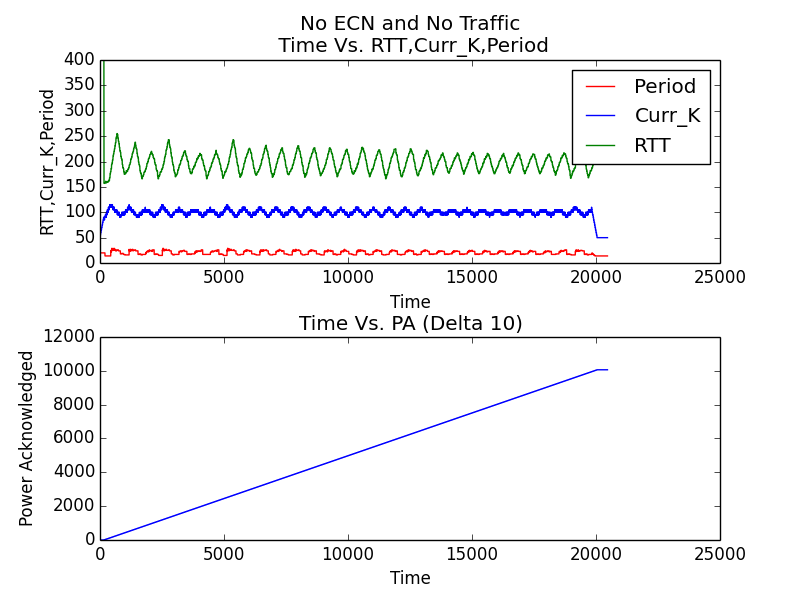
\includegraphics[width=0.50\textwidth]{Figures/iccps2014/no_ecn_no_tr_d10.png}
  \caption{No ECN, No Traffic, $\delta$ = 10}
  \label{fig:no_ecn_no_tr_d10}
    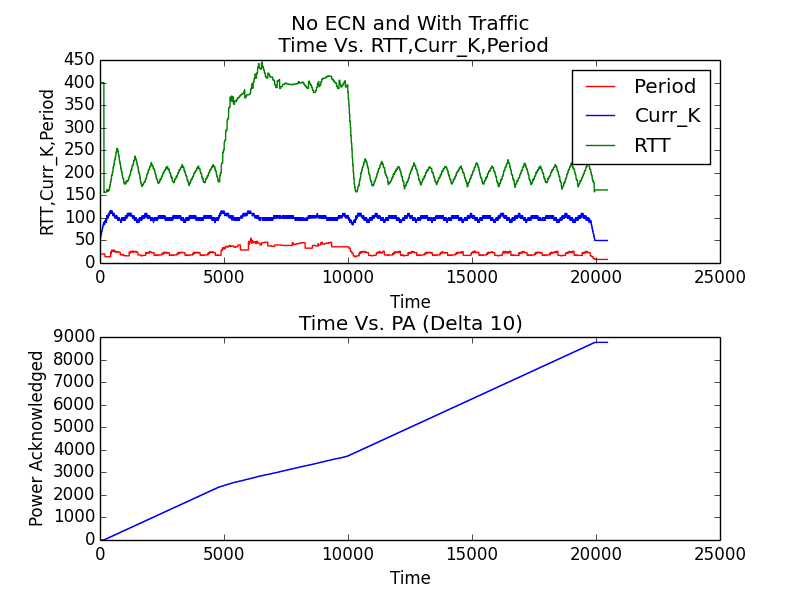
\includegraphics[width=0.50\textwidth]{Figures/iccps2014/no_ecn_w_tr_d10.png}
  \caption{No ECN, With Traffic, $\delta$ = 10}
  \label{fig:no_ecn_w_tr_d10}

  \end{center}
\end{figure}
%----------------------------------------
%----------------------------------------
\begin{figure}[htb]
  \begin{center}

    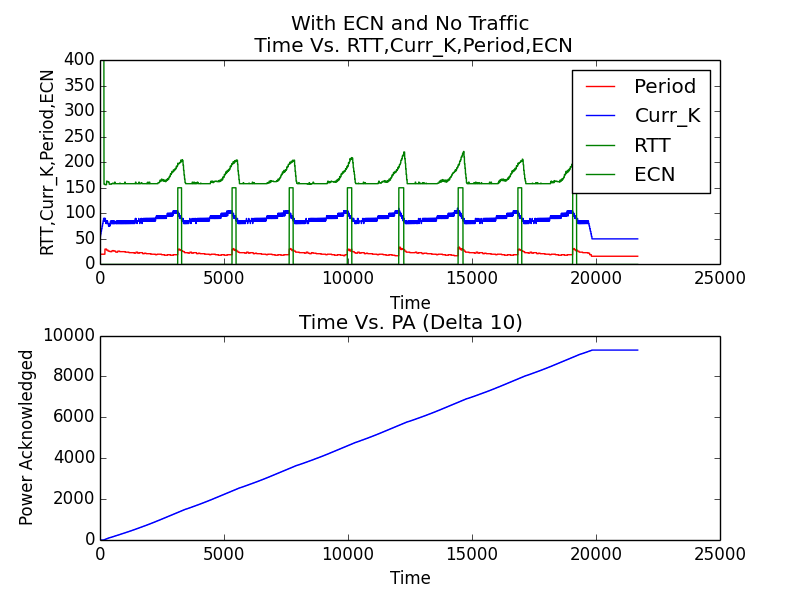
\includegraphics[width=0.50\textwidth]{Figures/iccps2014/w_ecn_no_tr_d10.png}
  \caption{With ECN, No Traffic, $\delta$ = 10}
  \label{fig:w_ecn_no_tr_d10}
    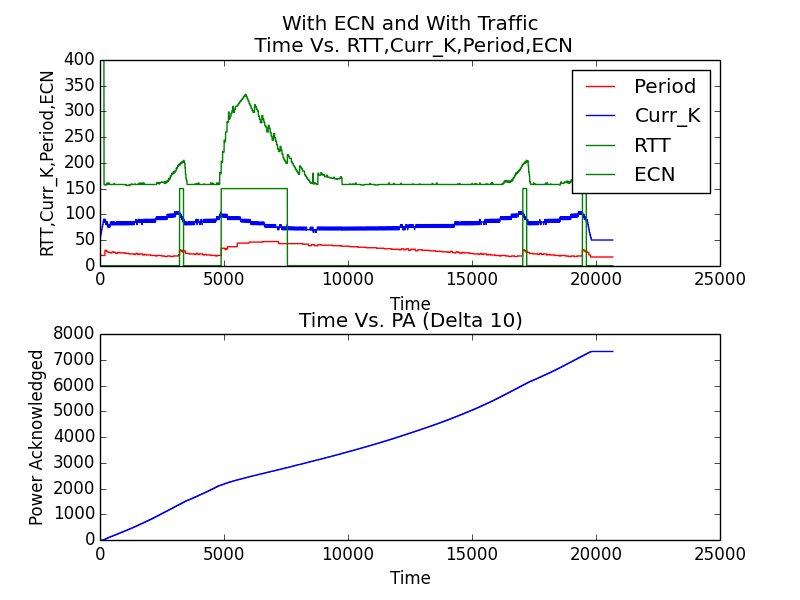
\includegraphics[width=0.50\textwidth]{Figures/iccps2014/w_ecn_w_tr_d10.png}
  \caption{With ECN, With Traffic, $\delta$ = 10}
  \label{fig:w_ecn_w_tr_d10}

  \end{center}
\end{figure}
%----------------------------------------
%----------------------------------------
\begin{figure}[htb]
  \begin{center}
  
    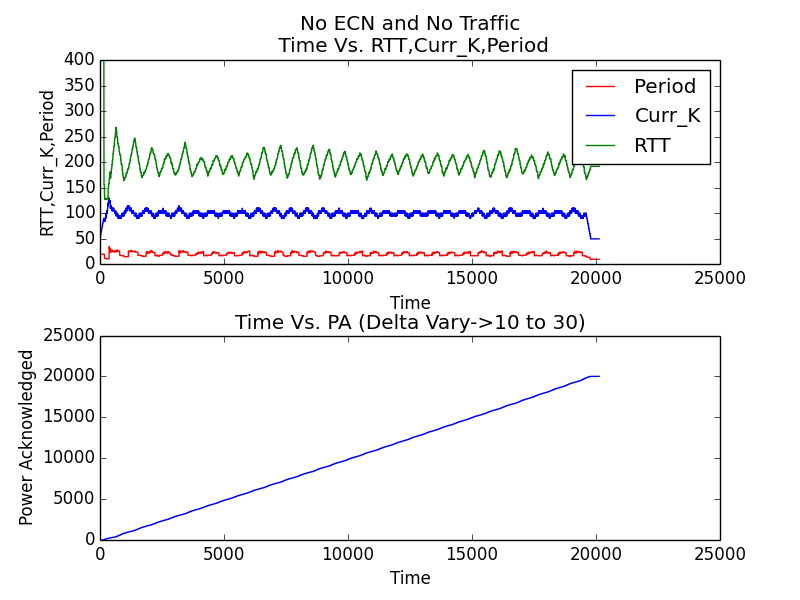
\includegraphics[width=0.50\textwidth]{Figures/iccps2014/no_ecn_no_tr_d10_30.png}
  \caption{No ECN, No Traffic, Vary $\delta$ 10 to 30}
  \label{fig:no_ecn_no_tr_d10_30}
    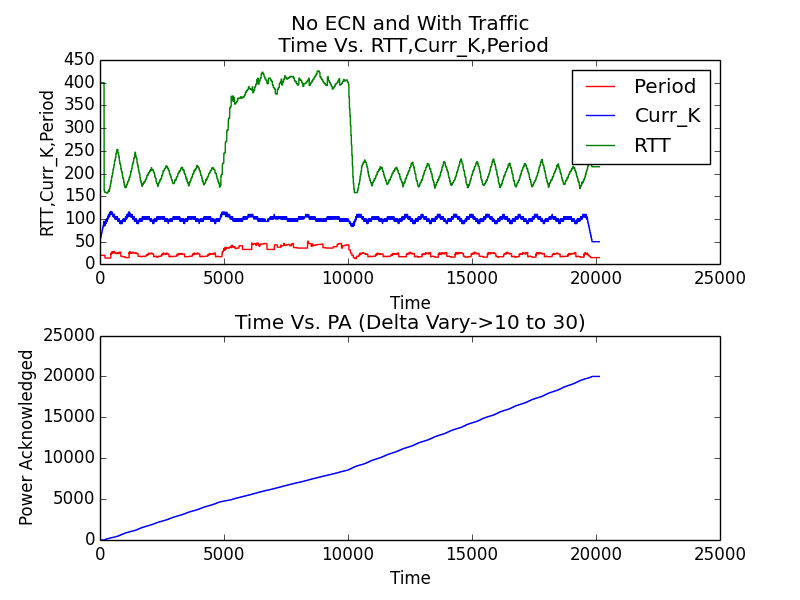
\includegraphics[width=0.50\textwidth]{Figures/iccps2014/no_ecn_w_tr_d10_30.png}
  \caption{No ECN, With Traffic, Vary $\delta$ 10 to 30}
  \label{fig:no_ecn_w_tr_d10_30}

  \end{center}
\end{figure}
%----------------------------------------
%----------------------------------------
\begin{figure}[htb]
  \begin{center}

    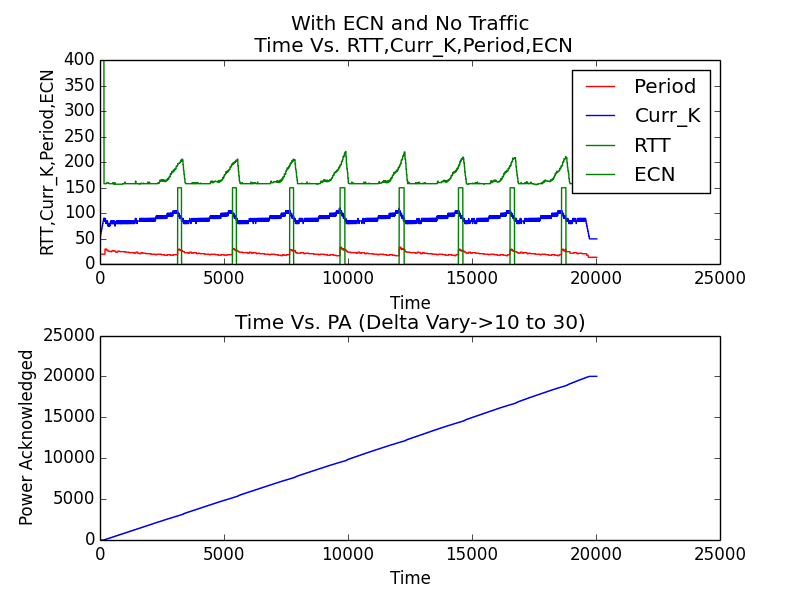
\includegraphics[width=0.50\textwidth]{Figures/iccps2014/w_ecn_no_tr_d10_30.png}
  \caption{With ECN, No Traffic, Vary $\delta$ 10 to 30}
  \label{fig:w_ecn_no_tr_d10_30}
    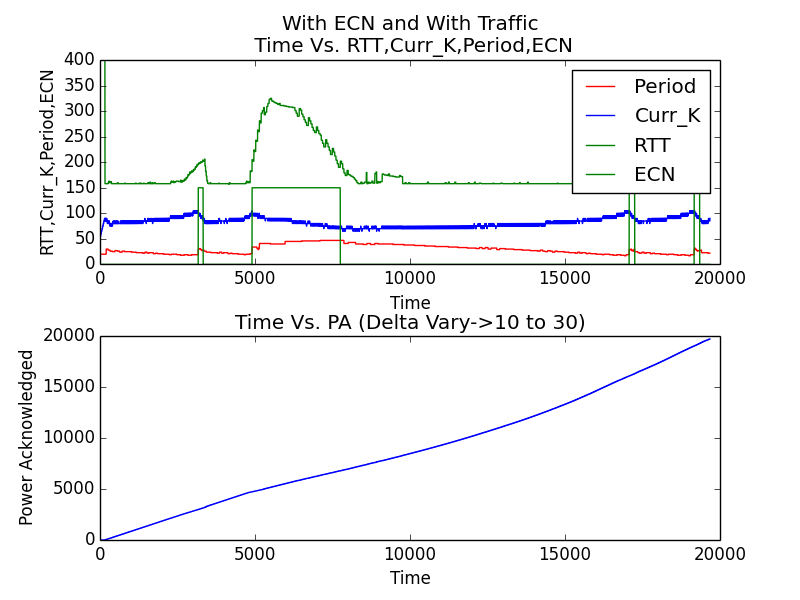
\includegraphics[width=0.50\textwidth]{Figures/iccps2014/w_ecn_w_tr_d10_30.png}
  \caption{With ECN, With Traffic, Vary $\delta$ 10 to 30}
  \label{fig:w_ecn_w_tr_d10_30}

  \end{center}
\end{figure}
%----------------------------------------











